\section{Introduction}
\label{section_intro}
The calculation of planetary orbits is arguably the canonical problem in mathematical physics.
Isaac Newton invented differential calculus while working on this problem, and used his theory of gravitation to solve it.
In the important special case that one body in the system is a dominant central mass,
and all other bodies are viewed as massless ``test particles,'' then a simple closed form solution is possible.
This formulation of the gravitational problem is often called the \href{https://en.wikipedia.org/wiki/Kepler_problem}{Kepler Problem},
named after \href{https://en.wikipedia.org/wiki/Johannes_Kepler}{Johannes Kepler}.
Kepler first studied this problem and published his famous \href{https://en.wikipedia.org/wiki/Kepler\%27s_laws_of_planetary_motion}{three laws of planetary motion},
the first of which states that the planets move in elliptical orbits with the Sun at one focus.
This is a surprisingly good approximation for the evolution of the Solar System, and the basis for the efficient linearized search over orbital elements developed in this thesis.

The two-body approximation is not, however, sufficiently accurate for a high precision model of the past and future positions of the known bodies in the Solar System.
While the mass of the Sun is much larger than the combined planetary mass, 
\footnote{Jupiter has a mass of $9.55 \times 10^{-4}$ of the Sun, and the Sun accounts for 99.8\% of the Solar System mass;
see \href{https://en.wikipedia.org/wiki/List_of_Solar_System_objects_by_size}{Wikipedia - Solar System objects}}
the planets are sufficiently massive (and often closer to each other and other bodies of interest) 
that gravity due to planets must also be accounted for.
The modern approach to determining orbits in the Solar System is to use numerical integrators of the differential equations of motion.

\section{The \tty{REBOUND} Library for Gravitational Integration}
\label{section_rebound}
\tty{REBOUND} is an open source library for numerically integrating objects under the influence of gravity.
It is available on GitHub at \href{https://github.com/hannorein/rebound}{github.com/hannorein/rebound}.
It is a first rate piece of software and I would like to thank Matt Holman and Matt Payne for recommending it to me last year.
At the end of Applied Math 225, I wrote a research paper in which I learned to use this library, 
extensively tested it on the Solar System, and used it to simulate the near approach of the asteroid Apophis to Earth that will take place in 2029.
In this thesis, I use \tty{REBOUND} as the ``gold standard'' of numerical integration.
Because of its important role, I describe below how the \tty{IAS15} integrator I selected works.
\footnote{\tty{REBOUND} provides a front end to use multiple integrators. In this project, I make exclusive use of the default \tty{IAS15} integrator.}

The \tty{IAS15} integrator, presented in a 2014 paper by Rein and Spiegel, is a an impressive achievement.
It a fast, adaptive, 15th order integrator for the $N$-body problem that is (amazingly!) 
accurate to machine precision over a billion orbits.  
The explanation is remarkably simple in comparison to what this algorithm can do.  
Rein and Spiegel start by writing the equation of motion in the form 
$$y'' = F[y', y, t]$$
Here $y$ is the position of a particle; $y'$ and $y''$ are its velocity and acceleration;
and $F$ is a function with the force acting on it over its mass.
In the case of gravitational forces, the only dependence of $F$ is on $y$; 
but one of the major advantages of this framework is its flexibility to support other forces,
including non-conservative forces that may depend on velocity.
Two practical examples are drag forces and radiation pressure.

This expression for $y''$ is expanded to 7th order in $t$, 
$$y''[t] \approx y_0'' + a_0t + a_1t^2 + \cdots +a_6 t^7$$
They next change variables to dimensionless units $h = t / dt$ and coefficients $b_k = a_k dt^{k+1}$:
$$y''[t] \approx y_0'' + b_0h + b_1h^2 + \cdots + b_6 h^7$$
The coefficients $h_i$ represent relative sample points in the interval $[0, 1]$ that subdivide a time step.
Rein and Spiegel call them substeps.  
The formula is rearranged in terms of new coefficients $g_k$ with the property that $g_k$ depends
only on force evaluations at substeps $h_i$ for $i \le k$,
$$y''[t] \approx y_0'' + g_1h + g_2h(h-h_1) + g_3h(h-h_1)(h-h_2) + \cdots + g_8 h (h-h_1) \cdots (h-h_7)$$
Taking the first two $g_i$ as examples and using the notation $y_n'' = y''[h_n]$,
$$g_1 = \frac{y_1'' - y_0''}{h_1} ,\quad\quad  g_2 = \frac{y_2'' - y_0'' -g_1h_2}{h_2(h_2-h_1)}$$
This idea has a similar feeling to \href{https://en.wikipedia.org/wiki/Jacobi_coordinates}{Jacobi coordinates}
in the N-body gravitational problem: a change of coordinates with a dependency structure to allow sequential computations.

Using the $b_k$ coefficients, it is possible to write polynomial expressions for $y'[h]$ and $y''[h]$:
\begin{align*}
y'[h] &\approx y_0' + h dt \left(y_0'' + \frac{h}{2}\left(b_0 + \frac{2h}{3}\left(b_1 + \frac{}{} \cdots \right)\right) \right) \\
y[h] &\approx y_0 + y_0' h dt + \frac{h^2dt^2}{2}\left(y_0'' + \frac{h}{3}\left(b_0 + \frac{h}{2}\left(b_1 + \frac{}{} \cdots \right)\right) \right)
\end{align*}

The next idea is to use \href{http://mathworld.wolfram.com/RadauQuadrature.html}{Gauss-Radau quadrature}
to approximate this integral with extremely high precision.  
Gauss-Radau quadrature is similar to standard Gauss quadrature for evaluating numerical integrals, 
but the first sample point is at the start of the integration window at $h=0$.
This is a strategic choice here because we already know $y'$ and $y''$ at $h=0$ from the previous time step.
This setup now reduces calculation of a time step to finding good estimate of the coefficients $b_k$.
Computing the $b_k$ requires the forces during the time step at the sample points $h_n$,
which in turn provide estimates for the $g_k$, and then feed back to a new estimate of $b_k$.

This is an implicit system that Rein and Spiegel solve efficiently using what they call a predictor-corrector scheme.
At the cold start, they set all the $b_k=0$, corresponding to constant acceleration over the time step.
This leads to improved estimates of the forces at the substeps, and an improved estimates for the path on the step.
This process is iterated until the positions and velocities have converged to machine precision.
The first two time steps are solved from the cold start this way.  

Afterwards, a much more efficient initial guess is made.  
They keep track of the change between the initial prediction of $b_k$ and its value after convergence,
calling this correction $e_k$.  At each step, the initial guess is $b_k$ at the last step plus $e_k$.
An adaptive criterion is used to test whether the predictor-corrector loop has converged.
The error is estimated as 
$$\widetilde{\delta b_6} = \frac{\max_i |\delta b_{6,i}|}{\max_i |y_i''|} \;.$$
The index $i$ runs over all 3 components of each particle.
The loop terminates when $ \widetilde{\delta b_6} < \epsilon_{\delta b}$; they choose $\epsilon_{\delta b} = 10^{-16}$.
It turns out that the $b_k$ behave well enough for practical problems that this procedure will
typically converge in just 2 iterations!

The stepsize is controlled adaptively with an analogous procedure.
The tolerance is set with a dimensionless parameter $\epsilon_b$,
which they set to $10^{-9}$.
As long as the step size $dt$ is ``reasonable'' in the sense that it can capture
the physical phenomena in question, the error in $y''$ will be bounded by the last term
evaluated at $h=1$, i.e. the error will be bounded by $b_6$.
The relative error in acceleration $\widetilde{b_6} = b_6 / y''$ is estimated as
$$ \widetilde{b_6} = \frac{\max_i |b_{6,i}|}{\max_i |y_i''|} \;.$$
These are similar to the error bounds for convergence of the predictor-corrector loop,
but involve the magnitude of $b_6$ rather than its change $\delta b_6$.
An immediate corollary is that changing the time step by a factor $f$ will change $b_6$
by a factor of $f^7$.

An integration step is computed with a trial step size $dt_{\text{trial}}$.
At the end of the calculation, we compute the error estimate $\widetilde{b_6}$.
If it is below the error tolerance $\epsilon_b$, the time step is accepted.
Otherwise, it is rejected and a new attempt is made with a smaller time step.
Once a time step is accepted, the next  time step is tuned adaptively according to
$dt_{\text{required}} = dt_{\text{trial}} \cdot \left( \epsilon_b / \widetilde{b_6}\right)^{1/7}$.
Please note that while the relative error in $y''$ may be of order 7, 
the use of a 15th order integrator implies that 
shrinking the time steps by a factor $\alpha$ will improve the error by a factor of $\alpha^{16}$.

\section{A Brief Review of the Keplerian Orbital Elements}
\label{section_orbital_elements}
In his work on the two-body problem and the orbits of the planets, Kepler defined 
\href{https://en.wikipedia.org/wiki/Orbital_elements}{orbital elements}
that are still in use today.
A set of orbital elements pertains to a body as of a particular instant in time, which is typically referred to as the ``epoch'' in this context.
The data sources I've seen all describe the time as a floating point number in the \href{https://en.wikipedia.org/wiki/Julian_day}{Modified Julian Day} (mjd) format.
In particular, I obtained orbital elements for all the known asteroids from \href{https://ssd.jpl.nasa.gov/?sb_elem}{JPL small body orbital elements}
as of MJD 58600.0, corresponding to 27-Apr-2019 on the Gregorian calendar.\\
Figure \ref{fig:KeplerianOrbitalElements} illustrates the six orbital elements.

\begin{figure}[h]
\begin{subfigure}[t]{0.5\textwidth}
\centering
\includegraphics[width=\linewidth]{../figs/web/orbital_elements_wikipedia.png}
\end{subfigure}
\hfill
\begin{subfigure}[t]{0.5\textwidth}
\centering
\includegraphics[width=\linewidth]{../figs/web/kepler_ellipse.png}
\end{subfigure}
\caption[Definition of the Traditional Keplerian Orbital Elements]
{Definition of the Traditional Keplerian Orbital Elements (courtesy of 
\href{https://en.wikipedia.org/wiki/Orbital_elements}{Wikipedia} and
\href{https://www.planetary.org/blogs/emily-lakdawalla/2012/3380.html}{planetary.org}).}
\label{fig:KeplerianOrbitalElements}
\end{figure}

\begin{samepage}
The names and conventional symbols for Keplerian elements are:
\begin{itemize}
\item $a$, the semi-major axis; a distance
\item $e$, the eccentricity; dimensionless
\item $i$, the inclination; an angle
\item $\Omega$, the longitude of the ascending node; an angle
\item $\omega$, the argument of perihelion; an angle
\item $f$, the true anomaly; an angle
\item $M$, the mean anomaly; an angle
\item $t_0$, the epoch; a time
\end{itemize}
\end{samepage}
The parameters $a$ and $e$ define the size and shape of the orbital ellipse.
The three angles $i$, $\Omega$, and $\omega$ define its orientation in a three dimensional reference frame.
The true anomaly $f$ or mean anomaly $M$ define where the orbiting body is in its orbital ellipse as of the epoch.
Distances are in A.U. in both JPL and \tty{REBOUND}.  \\
Angles are quoted in degrees in JPL and in radians in \tty{REBOUND}.\\
The epoch is represented as a Modified Julian Date.

These orbital elements have stood the test of time because they are useful and intuitive.
They are ideal for many computations, both theoretical and numerical, because in the case of the two-body problem, five of the six orbital elements remain constant.
Perhaps equally useful, in an N-body system with a centrally dominant mass including our Solar System,
the first five elements change very slowly, while the mean anomaly changes approximately linearly in time.
These two properties make orbital elements ideal for splining interpolated positions and velocities.
This approach is used in the generation of \href{https://en.wikipedia.org/wiki/Ephemeris}{ephemerides} from numerical integrations of the Solar System.

The careful reader will note that there are 8 entries in the table above, but I've described elements as coming six at a time.
The epoch $t_0$ is considered to be the ``seventh element'' because in the Kepler two-body problem, we can describe one body at different times, but it will have the same orbit.
This point of view extends to the N-body problem, which is fully reversible; the same system can be described as of different moments in time.
In practice, the orbital elements are often used to describe the initial conditions of all the bodies for an integration.
The problem is then integrated numerically, possibly both forwards and backwards.
Orbital elements can be reported for any body of interest.

A body orbiting the Sun has six degrees of freedom.  
In Cartesian coordinates, there are three for the position and three for the velocity.
In orbital elements, the first five are almost always $(a, e, i, \Omega, \omega)$.
These five will remain constant for a body moving in the Kepler two-body problem.

There is some variation in the choice of the sixth element, because different representations have different advantages.
The true anomaly $f$ is most convenient for transforming from orbital elements to Cartesian space.
The mean anomaly $M$ is most convenient for studying the time evolution of the system, because it changes linearly with time in the Kepler two-body problem.
The \href{https://en.wikipedia.org/wiki/Eccentric_anomaly}{eccentric anomaly} $E$ is yet another angle describing a body in orbit.
Figure \ref{fig:OrbitalAnomalies} depicts the three orbital anomalies.
The mean anomaly and eccentric anomalies are related by the famous 
\href{https://en.wikipedia.org/wiki/Kepler\%27s_equation}{Kepler's Equation},
shown below along with the transformation between $E$ and $f$
\begin{align*}
M &= E - e \sin(E) & \textrm{Kepler's Equation} \\
\tan \left(\frac{f}{2} \right) &= \sqrt{\frac{1+e}{1-e}} \cdot \tan \left( \frac{E}{2} \right) &\textrm{true to eccentric}
\end{align*}

\begin{figure}
\begin{center}
\includegraphics[width=0.40\textwidth]{../figs/web/orbital_anomalies.png}
\end{center}
\caption[Three Orbital Anomalies: Eccentric ($E$), Mean ($M$) and True ($f$)]
{Three Orbital Anomalies: Eccentric, Mean and True}
\label{fig:OrbitalAnomalies}
\end{figure}
 
The linear evolution of the mean anomaly, along with Kepler's equation, allows us to efficiently compute orbits for the Kepler two-body problem.
The relationship between the eccentric anomaly $E$ and true anomaly $f$ is a one to one function that can be evaluated fast on a computer.
The mapping from eccentric anomaly $E$ to mean anomaly $M$ is also fast.
The inverse mapping from $M$ to $E$ does not have a known analytical form.
But it can be evaluated rapidly using Newton's Method with a reasonable initial guess.
This is the method that I use to compute the orbits under the Kepler approximation. 

\section{Numerical Integration of the Planets in \tty{REBOUND}}
\label{section_numerical_integration}
I have described above a library \tty{REBOUND} that can efficiently integrate the Solar System.
Data for the initial conditions can obtained from \href{https://ssd.jpl.nasa.gov/?horizons}{Horizons},
a service provided by the Jet Propulsion Laboratory (JPL) at NASA that is free to the public.
In principle, integrating the Solar System is a straightforward exercise.
In practice, there are quite a few details that need to be worked out before you can obtain reliably correct answers.
You must pay attention to units and the frame of reference.
You also need to carefully specify the bodies you submit to Horizons.
Horizons has separate identifiers for e.g. the barycenter of the Earth-Moon system, the Earth, and the Moon.

The module \tty{horizons.py} contains functions used to query the Horizons API.
It also maintains a local cache with the results of prior queries; 
this yields significant savings in time because a typical horizons query using the Horizons API in \tty{REBOUND} takes about one second.
The main function in this module is \tty{make\_sim\_horizons}.
Given a list of object names and an epoch, it queries Horizons for their positions and velocities as of that date.
It uses this data to instantiate a \tty{REBOUND Simulation} object. \\
The module \tty{rebound\_utils.py} contains functions used to work with \tty{REBOUND} simulations.
It includes functions to build a simulation (\tty{make\_sim}).
This will seek to load a saved simulation on disk if it is available, otherwise it will query Horizons for the required initial conditions.
The function \tty{make\_archive} builds a \tty{REBOUND SimulationArchive}.
As the name suggests, a \tty{SimulationArchive} is a collection of simulation snapshots that  have been integrated.
This function also saves the integrated positions of the planets and test bodies as plain old \tty{numpy} arrays for use in downstream computations.

The module \tty{planets.py} performs the numerical integration of the planets.
To be more precise, it will integrate four different collections of massive bodies in the Solar System
\footnote{Masses of Solar System objects were obtained from \href{https://en.wikipedia.org/wiki/List_of_Solar_System_objects_by_size}{Wikipedia - Solar System objects}.
The module \tty{solar\_system\_objects.py} includes object names, masses, and Horizons integer IDs.}
\begin{itemize}
\item \textbf{Planets}: The Sun; The Earth and Moon as separate bodies; and the barycenters of the other seven IAU planets 
Mercury, Venus, Mars, Jupiter, Saturn, Uranus, and Neptune (10 objects)
\item \textbf{Moons}: The 8 IAU planets, plus the following significant moons and Pluto (31 objects): \\
Earth: Moon (Luna)\\
Jupiter: Io, Europa, Ganymede, Callisto \\
Saturn: Mimas, Enceladus, Tethys, Dione, Rhea, Titan, Iapetus, Phoebe \\
Uranus: Ariel, Umbriel, Titania, Oberon, Miranda \\
Neptune: Triton, Proteus \\
Pluto: Charon 
\item \textbf{Dwarfs}: Selected objects in the Solar System with a mass at least $10^{-10}$ Solar masses (31 objects): \\
Planets: Earth, Moon, and barycenters of the other seven IAU planets \\
Above $10^{-9}$: Pluto Barycenter, Eris, Makemake, Haumea \\
Above $10^{-10}$: 2007 OR10, Quaoar, Hygiea, Ceres, Orcus, Salacia, Varuna, Varda, Vesta, Pallas
\item \textbf{All}: All objects in the Solar System with a mass at least $10^{-10}$ Solar masses (45 objects): \\
All 8 IAU planets (not barycenters) \\
All the heavy moons above \\
All the dwarf planets and heavy asteroids above
\end{itemize}

Each configuration above was integrated for a 40 year period spanning 2000-01-01 to 2040-12-31 and a time step of 16 days.
I tested the integration by comparing the predicted positions of the 8 planets to the position quoted by Horizons at a series of test dates.
The test dates are at 1 year intervals over the full 40 year span that is simulated.
The best results were obtained by integrating the smallest collection: Earth, Moon, and the barycenters of the other 7 planets.
I was a bit surprised at this result and expected to do slightly better as the collection of objects became larger.
Position errors are reported in AUs, with the root mean square (RMS) error over the 40 annual dates.
I also compute an angle error by comparing the instantaneous direction from each planet to Earth geocenter in the BME frame.
I reported errors on this basis because on this problem, everything is done in terms of directions so precision eventually
comes down to a tolerance in arc seconds.

\begin{table}
\centering
{
\begin{tabular}{ | c | c | c |}
\hline
\multicolumn{1}{|p{2cm}|}{\centering Object \\ Collection } & 
\multicolumn{1}{|p{2cm}|}{\centering Position \\ Error \\ AU} & 
\multicolumn{1}{|p{2cm}|}{\centering Angle \\ Error \\ ArcSec} \\
\hline
Planets & $5.38 \times 10^{-6}$ & 0.79 \\
Moons & $1.35 \times 10^{-5}$ & 0.81 \\
Dwarfs & $5.38 \times 10^{-6}$ & 0.79\\
All & $1.35 \times 10^{-5}$ & 0.81 \\
\hline
\end{tabular}
\caption[Root Mean Square Error in Integration of Planets vs. Horizons]
{Root Mean Square Error in Integration of Planets vs. Horizons\\
Position Error: RMS error of 8 planets in AU.\\
Angle Error: RMS error in direction from planet to Earth geocenter, in Arc Seconds}
}
\label{tbl:PlanetIntegrationError}
\end{table}

While it might at first seem surprising that the results are worse for the more complex integrations including the moons,
it's important to realize that this problem is intrinsically more difficult.
Simulating the evolution of the barycenter of e.g. the Jupiter system is significantly easier than keeping track of the heavy moons and integrating them separately.
Overall these results are excellent; over a span of 20 years in either direction, integrations are accurate on the order of $10^{-6}$ AU.
\footnote{For readers less familiar with astronomy, one AU (astonomical unit) is a unit of length that was defined to match the mean distance from the Earth to the Sun.
It is official defined as equal to 1.495 878 707 E11 meters; see \href{https://en.wikipedia.org/wiki/Astronomical_unit}{Wikipedia - Astronomical Unit}.
It is extremely convenient for Solar System integrations since it leads to distances on the scale of around 1 to 10, 
and for this reason it is the default distance unit in \tty{REBOUND}.}
The angular precision on the order of $\sim 0.8$ arc seconds is also excellent for such a long time span and well within the tolerance of this application.

After reviewing these results, I decided that the optimal strategy for the asteroid search problem was to treat the heavy bodies 
in the Solar System as the smallest collection, shown on row 1.
It is necessary to model the position of the Earth and Moon separately rather than the Earth-Moon barycenter, 
since our observatories are on the planet, not relative to the planetary system barycenter.
However, the role of the other planets is only as a gravitational attractor that deflects the orbit of the Earth and the asteroids.
Speed is important in this application, so the smallest and fastest collection was the clear choice.

The second test of the integration extends the bodies under consideration from the planets to include ten test asteroids.
I selected as the test asteroids the first 10 IAU numbered asteroids: Ceres, Pallas, Juno, Vesta, Iris, Hygiea, Egeria, Eunomia, Psyche, Fortuna.
This test does not yet exercise the part of the code that instantiates asteroid orbits based on the bulk orbital elements files; that comes later.
The asteroids here are initialized the same way as the planets, by querying the Horizons API in \tty{REBOUND}.
The test protocol here was the same as for the planets.
I compared the positions of these asteroids in the barycentric mean ecliptic frame predicted by my integration at annual dates to the positions quoted by JPL.
I also compared the instantaneous angle from Earth geocenter to the asteroid.

Figure \ref{fig:AsteroidIntegrationErrorHorizons} summarizes the results.
If we focus on a plausible window of $\pm 5$ years around 2020, we can see that the selected planets integration is extremely accurate.
Angular errors 5 years out are on the order of $0.5$ arc seconds.\\
The charts and numerical outputs can be obtained at the command line by running
\begin{lstlisting}[style=CodeSnippet]
(kepler) $ python planets.py --test
\end{lstlisting}
(\tty{kepler} is the name of the Anaconda environment with the necessary dependencies installed.
An anaconda environment file \tty{kepler.yml} is included in the \tty{env} directory of the Git 
\href{https://github.com/memanuel/kepler-sieve}{repository}.)
\begin{figure}[hbt!]
\begin{center}
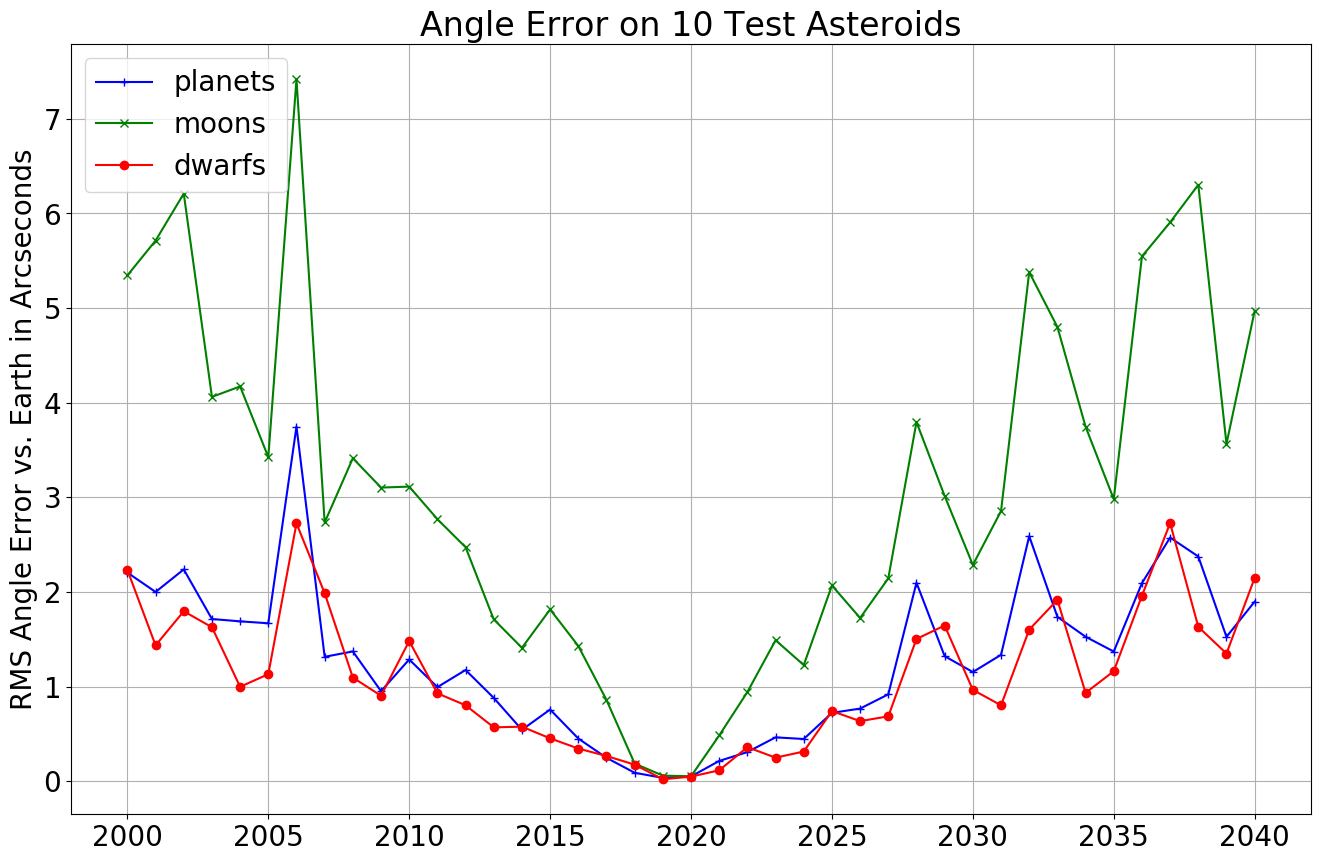
\includegraphics[width=1.0\textwidth]{../figs/integration_test/planets/sim_pos_error_comp.png}
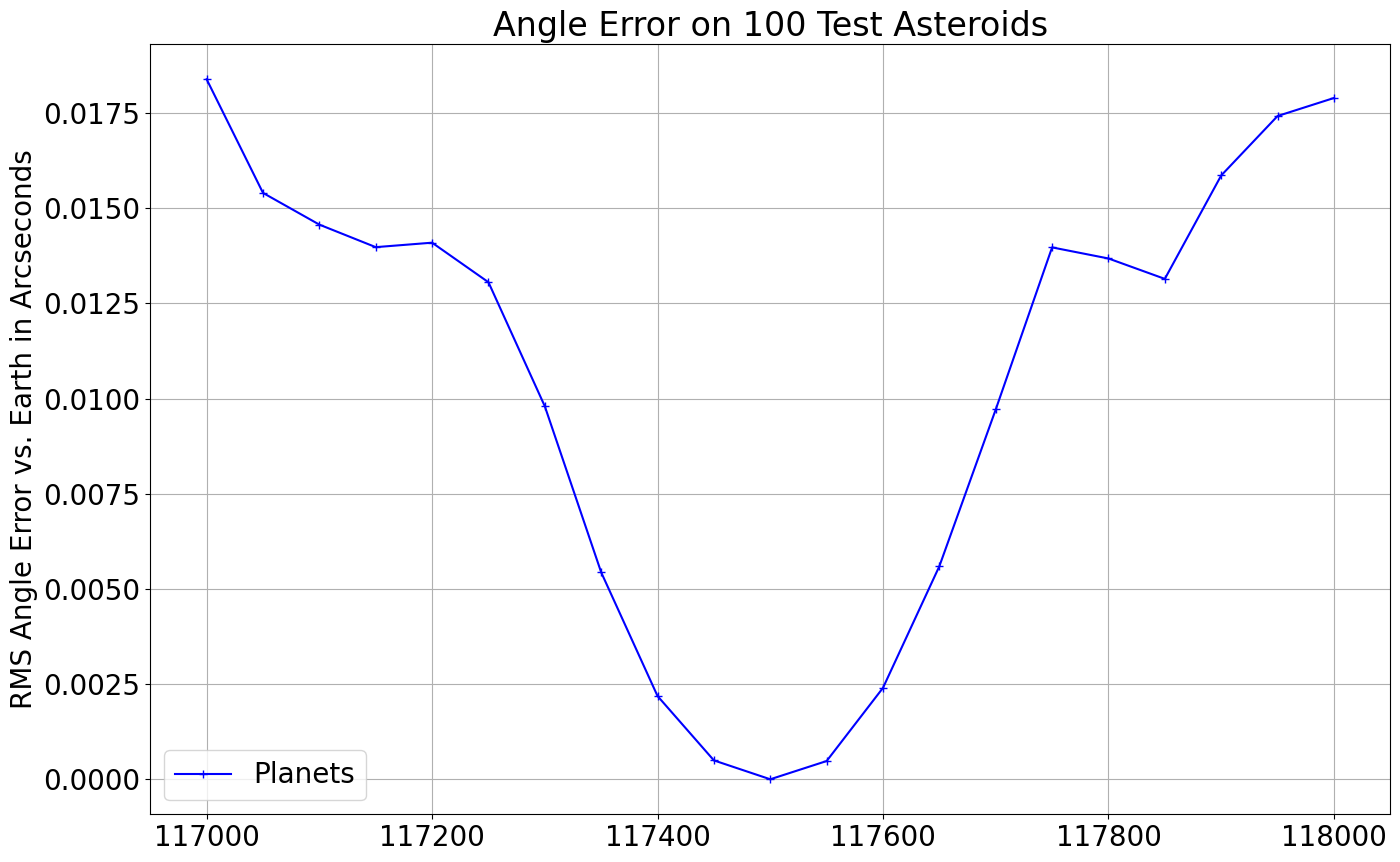
\includegraphics[width=1.0\textwidth]{../figs/integration_test/planets/sim_ang_error_comp.png}
\end{center}
\caption[Position and Angle Error of 10 Test Asteroids Initialized from Horizons]
{Position and Angle Error of 10 Test Asteroids. \\
My integration is compared to positions extracted from Horizons at 40 dates from from 2000 to 2040.\\
Initial conditions of the planets and asteroids are taken from the Horizons API as of MJD 58600 (2019-04-27).}
\label{fig:AsteroidIntegrationErrorHorizons}
\end{figure}

\section{Efficient Integration of All Known Asteroids}
\label{section_integrate_known_asteroids}
In the previous section I have described how to integrate the Sun and Planets where the initial conditions
are obtained from Horizons using the API included in \tty{REBOUND}.
While this is a reliable and simple procedure that is ideal if you have only a few bodies to integrate,
there is too much overhead in querying the Horizons API for it to be feasible for integrating all known asteroids.
(If you spent 1 second on each of the 733,489 asteroids with available data, 
you would sit at your computer for over 9 days waiting for the job to complete,
which it probably wouldn't because the angry folk at JPL would have probably blacklisted your IP address
for spamming their server.)
Horizons includes two data files available at \href{https://ssd.jpl.nasa.gov/?sb_elem}{Small-Body Elements}
that are intended for bulk integrations and large scale analysis.
The first two of these contain orbital elements for asteroids:
\begin{itemize}
\item Orbital elements for 541,128 asteroids with IAU numbers as of epoch 58,600
\item Orbital elements for 255,518 asteroids with designations but without IAU numbers; 
most elements have been updated to epoch 58,600, but some are older
\end{itemize}
I performed a bulk integration of the orbits of all 733,489 of these asteroids that had orbital elements as of the epoch 58600.
In principle, I could have integrated all of the remaining asteroids with older elements forward in time to 58,600, but I had to draw the line somewhere.
I took the fact that JPL didn't bother updating these older elements as evidence it wasn't a worthwhile use of time.

The module \tty{asteroid\_element.py} contains functions for working with the orbital elements in these two data files.
JPL follows different conventions than the defaults in \tty{REBOUND}.
Here is a brief comment about the columns used
\begin{itemize}
\item \textbf{Num} is the IAU asteroid number; only available in the numbered asteroid file
\item \textbf{Name} is the official IAU name; only available in the numbered asteroid file
\item \textbf{Designation} is the designation of known asteroids without IAU numbers
\item \textbf{a} is the semi-major axis in AU
\item \textbf{e} is the eccentricity (dimensionless)
\item \textbf{i} is the inclination $i$ quoted in degrees
\item \textbf{w} is the argument of periapsis $\omega$ in degrees
\item \textbf{Node} is the longitude of the ascending node $\Omega$ in degrees
\item \textbf{M} is the mean anomaly $M$ quoted in degrees
\item \textbf{H} is the $H$ parameter (mean brightness) in the H-G model of asteroid magnitude 
\footnote{\href{https://www.britastro.org/asteroids/dymock4.pdf}{BAA H-G Magnitude System} }
\item \textbf{G} is the $G$ parameter (sensitivity of brightness to phase angle)
\item \textbf{Ref} is the name of a JPL reference integration
\end{itemize}

Figure \ref{fig:OrbitalElementsDataFrame} shows the asteroid orbital elements as a Pandas DataFrame:
\begin{figure}[hbt!]
\begin{center}
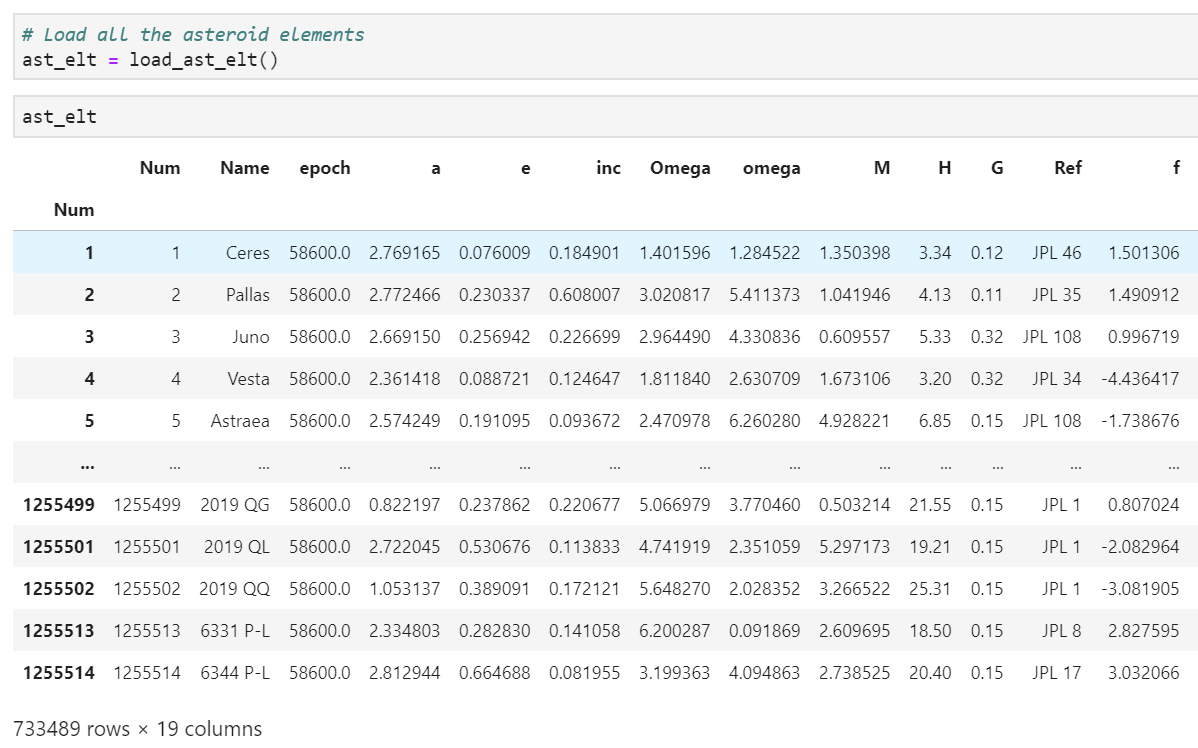
\includegraphics[width=1.0\textwidth]{../figs/elts/ast_elt_dataframe.png}
\end{center}
\caption[Orbital Elements of 733,489 Asteroids Downloaded from Horizons]
{Orbital Elements of 733,489 Asteroids Downloaded from Horizons.\\
I have calculated the true anomaly $f$ in \tty{REBOUND}.}
\label{fig:OrbitalElementsDataFrame}
\end{figure}
% \clearpage
To use these elements in \tty{REBOUND} is straightforward.
Converting angles from degrees to radians is trivial.
Distances are already quoted in AU.
Converting from a mean anomaly $M$ to a true anomaly $f$ is not an obvious operation.
Fortunately \tty{REBOUND} allows you to instantiate an orbit with any legal combination of six elements,
so I build the orbits from $M$ and save a copy with $f$. \\
The code to load the quoted orbital elements from JPL is in \tty{load\_ast\_elt} in \tty{asteroid\_element.py}.
The function \tty{load\_data\_impl} simply builds a Pandas DataFrame with all of the quoted elements.
The function \tty{ast\_data\_add\_calc} adds the computed true anomaly $f$.

There is one critical point to understanding these elements which is not at all obvious, so I will spell it out here.
When quoting orbital elements of a body, they are always in reference to a dominant central mass, called the ``primary''.
While it is often clear from the context what that mass is, it is not always.
In particular, two sound choices for the orbital elements of an asteroid are
\begin{samepage}
\begin{itemize}
\item The central mass is the Sun
\item The central mass is the Solar System barycenter
\end{itemize}
\end{samepage}
JPL quotes the asteroid orbital elements relative to the Sun, not the Solar System barycenter.
If you just plug in these elements to \tty{REBOUND} without specifying a primary, 
it will default to the center of mass of all the massive bodies in the simulation that have been entered prior.
This leads to a subtle error on the order of $10^{-3}$ that still wreaks havoc at the precisions required here.
Here are the most important lines of code to add each asteroid to the simulation:
\begin{lstlisting}[style=CodeSnippet]
sim_base = make_sim_planets(epoch_dt=epoch_dt)
primary = sim.particles[`Sun']
sim.add(m=0.0, a=a, e=e, inc=inc, Omega=Omega, omega=omega, M=M, primary=primary)
\end{lstlisting}

The code to integrate all the known asteroids is in \tty{asteroid\_integrate.py}.
At the risk of stating the obvious, when integrating asteroids, they are treated as massless ``test particles.''
That is, they move under the influence of gravity from the massive particles in the simulation (here, the Sun, Moon and Planets),
but they are \textit{not} modeled as having their own gravity.
This is an essential computational simplification.
$N$ massive bodies have ${N}\choose{2}$ gravitational interactions, so the cost of integrating them scales as $N^2 / 2$.
If you add $K$ massless bodies to the system, there are an additional $N\cdot K$ interactions, so the cost scales as $N^2 / 2 + N \cdot K$.
I broke the asteroids into chunks of $K=1000$, and used a collection of massive bodies with $N=10$ (Sun, 8 Planets, Moon).
A naive integration that treated them all as objects with gravitation that ``just happened to be equal to zero'' would cost $509,545$ calculations per time step.
The efficient treatment by \tty{REBOUND} of the asteroids as test particles reduces this cost to $10,045$, a savings of a factor of 488 (roughly $K/2$).

\tty{make\_sim\_asteroids} builds a \tty{REBOUND} simulation initialized with the elements of asteroids with numbers in a given range.
\tty{calc\_ast\_pos\_all} is the workhorse that integrates this simulation forward and backward in time over the requested date range.
It saves a \tty{REBOUND} simulation archive that allows the simulation to be loaded as of any time between the start and end.
It also saves \tty{numpy} arrays with the position and velocity of all the particles in the integration.
As before, all asteroids had their motions integrated over a 40 year period spanning 2000 to 2040.
The simulation archive is saved with an interval of 16 days; it will recover any requested date by performing 
a ``short hop'' integration from the nearest saved date.
The \tty{numpy} arrays are saved daily, because the intended use case is a direct cubic spline interpolation of positions and velocities.
\footnote{Splining orbital elements is more accurate and would allow for smaller splines, but I did not want to reinvent the wheel
of building an ephemeris library.}
Even with all of the computational efficiency of \tty{REBOUND}, this is a big computational job.
According to the time stamps of the output files, running it took about 4:30 (four and a half hours); 
this was redlining a server with 40 high-end Intel CPUs and 256 GB of RAM.
The size of the data saved is 1.37 TB.  
(The \tty{REBOUND} simulation archive is a fairly bulky format compared to the plain old data array; 
it's saving a lot of auxiliary information that is required to efficiently restart the simulation anywhere.)
I ended up saving it to a network attached storage device on my network so it didn't overflow the main file system on the server where the job was running.

I tested the accuracy of this integration using a similar approach to the integration of the planets.
I extracted the positions and velocities of 25 test asteroids from the Horizons API.
The test asteroids were the first 25 numbered asteroids, starting with Ceres and ending with Phocaea.
Comparisons were made at annual intervals in the 40 year period.
I call this the ``soup to nuts'' test of the asteroid integration.
While it might look the same as the previous test of the asteroid integration, there is an important difference.
The asteroids on the last test had their initial conditions determined by querying the same Horizons API.
This time, only the initial conditions of the massive bodies were taken from Horizons.
Initial conditions for the asteroids were based on the orbital elements in the two JPL files described above.\\
This test can be run from the command line by typing
\begin{lstlisting}[style=CodeSnippet]
(kepler) $ python asteroid_integrate --test
\end{lstlisting}
The real program is run from the command line with different arguments, e.g. 
\begin{lstlisting}[style=CodeSnippet]
(kepler) $ python asteroid_integrate 10000 1000
\end{lstlisting}
would integrate a block of 1,000 asteroids starting at number 10,000. 
Figure \ref{fig:IntegrationTestAsteroidsFromElements} has two charts
presenting the root mean square position error and angle error to Earth geocenter for the 25 test asteroids.
\begin{figure}[hbt!]
\begin{center}
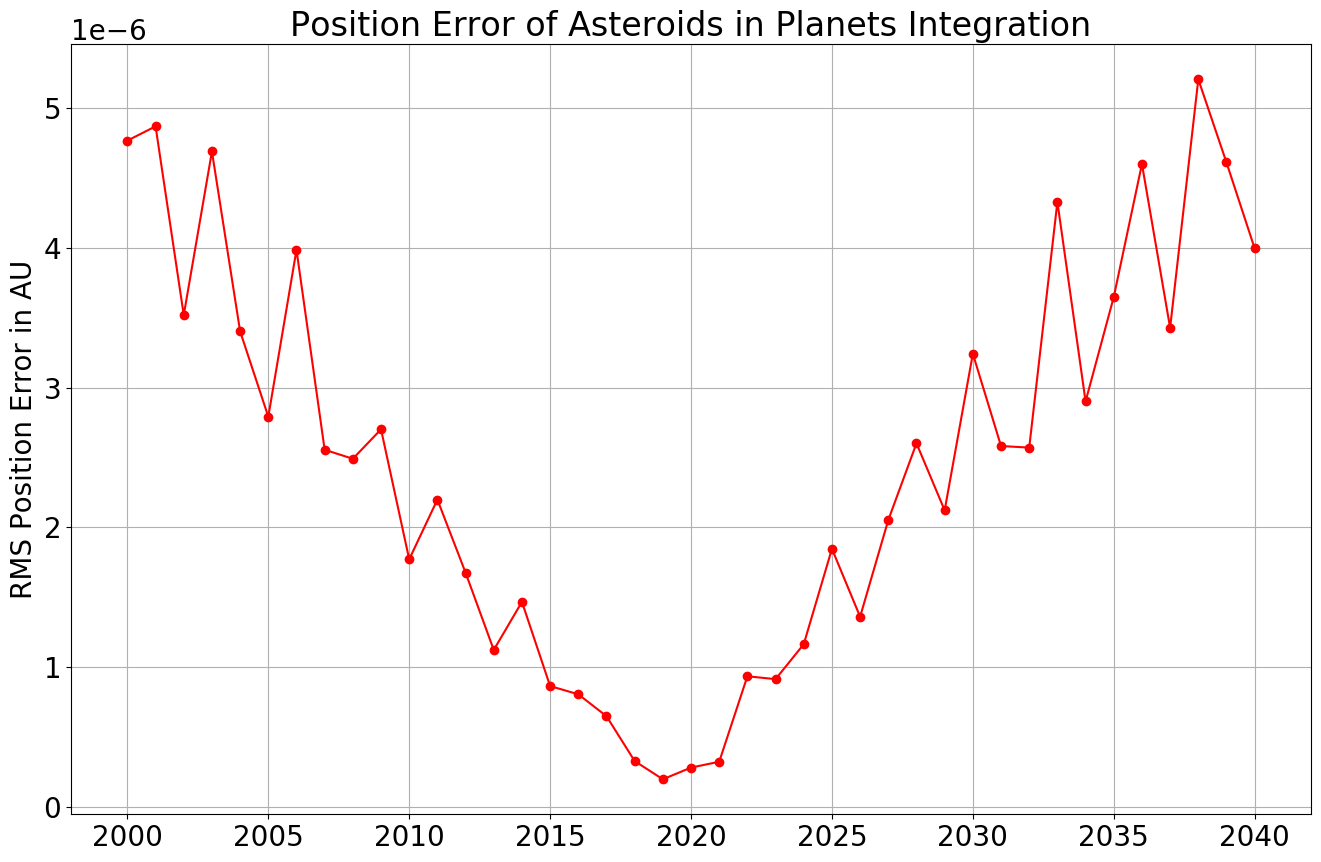
\includegraphics[width=0.95\textwidth]{../figs/integration_test/asteroids/sim_error_planets_asteroids_pos.png}
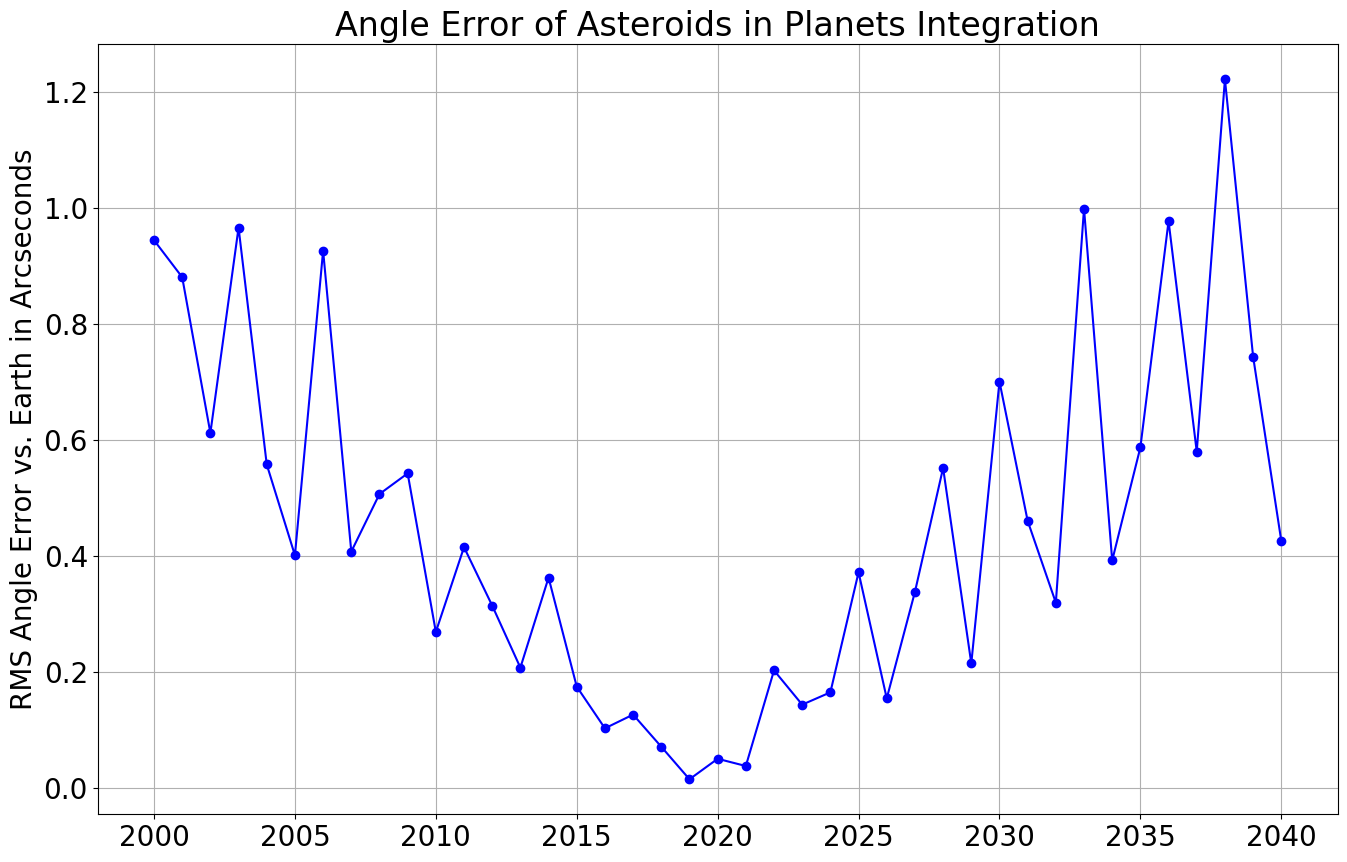
\includegraphics[width=0.95\textwidth]{../figs/integration_test/asteroids/sim_error_planets_asteroids_angle.png}
\end{center}
\caption[Position and Angle Error of 25 Test Asteroids]
{Position and Angle Error of 25 Test Asteroids\\
My integration is compared to positions extracted from Horizons at 40 dates from from 2000 to 2040.\\
Initial conditions of the planets are taken from the Horizons API as of MJD 58600 (2019-04-27). \\
Initial conditions of the asteroids are taken from orbital elements quoted in the 
Horizons small body elements file download as of MJD 58600.}
\label{fig:IntegrationTestAsteroidsFromElements}
\end{figure}
\clearpage

I was pleased with these results.
Over a 40 year span, the error is at worse on the order of $5 \times 10^{-6}$ AU, with a RMS of $2.49 \times 10^{-6}$ AU.
The angle errors over the full span have an RMS of 0.45 arc seconds,
and peak around 1.0 arc second for dates 20 years in the past or future.
In a more plausible 5 year band surrounding the epoch, accuracy is on the order of 0.2 arc seconds or better.
Here is one anecdotal data point to put this degree of precision in context.
On an earlier iteration, I foolishly did all calculations in the heliocentric rather than the barycentric frame.
I was confused because the orbital elements were quoted in the heliocentric frame.
When I finally switched to doing the computations in the barycentric frame 
(using the heliocentric elements only as a quotation mechanism for the initial conditions of the asteroids)
I improved the accuracy by about 0.6 arc seconds.

To summarize this section: I have presented an efficient and high precision integration of almost all the known objects in the Solar System.
The only dependency on Horizons in this calculation is the initial conditions of the Sun, Moon, and Planets.
Over a span of 40 years this integration is accurate on the order of $2.5 \times 10^{-6}$ AU of position and 0.45 arc seconds of angle to Earth.

I would like to take a step back here to comment on the progress that has been made in scientific computing and open source software
that makes it possible for one person to perform such a large scale computation.
When computations like this were first performed by NASA, they occurred on mainframes that were so expensive only the largest 
and best capitalized organizations could afford to buy them.
They cost millions to tens of millions of dollars in today's money.
Software to run these simulations was laboriously written and debugged, typically in \tty{FORTRAN}, dating back to an era when programs ran on punch cards.
\footnote{The film \href{https://en.wikipedia.org/wiki/Hidden_Figures}{Hidden Figures} paints an evocative portrait of this era
from the perspective of three black women whose contributions to the U.S. space program were only belatedly recognized.}
As recently as the 1980s and 1990s, the task of integrating the orbits of 733,000 asteroids could realistically be undertaken by only a small
handful of people with access to mainframe computers and extensive experience in both software engineering and mathematical physics.

Fast forward to today.  
High performance hardware is affordable and ubiquitous.
Open source software has made a state of the art numerical integrator freely available to the public.
NASA generously shares a treasure trove of valuable information along with excellent and user friendly APIs.
A single motivated individual with a strong undergraduate background in physics and programming,
but without specialized graduate level training, could plausibly have followed all the same steps shown here.
I find that a truly remarkable achievement of the scientific community.

\section{Integration of the Kepler Two Body Problem in TensorFlow}
\label{section_kepler_two_body_tensorflow}
In the previous section we have seen how to efficiently perform a numerical integration of the asteroids (or indeed any set of candidate elements).
But for the search technique presented here to work, we require a much faster integration that is also differentiable.
The integration algorithm used will be the analytical solution to the Kepler two-body problem.
An efficient high speed implementation of this algorithm on GPU, including derivatives, is done in TensorFlow.

I will begin with a brief review of the analytical solution of the Kepler two-body problem.
This derivation loosely follows the treatment given at \href{https://en.wikipedia.org/wiki/Kepler_problem}{Wikipedia - Kepler Problem},
but I have added significant explanations and intermediate steps because I found the article too terse to fully follow it.
A mathematically rigorous treatment of this subject can be found in \cite{MMCM}.
\footnote{See Chapter 2, section 8: Investigation of motion in a central field, and section 9: The motion of a point in three-space.}
The assumption that the orbiting body is infinitesimally light compared to the central mass is often translated to a model 
where the body moves in a central attractive field exerting a radial force $F(r)$ that always pulls towards the origin.
Because this force is radial, it does not change the angular momentum vector $\mathbf{L} = m\mathbf{v} \times \mathbf{r}$, 
which is a constant of the motion.
As we recall from high school physics, a body with angular velocity $\omega$ has tangential velocity $\omega r$
and centripetal acceleration $\omega^2 r$.
\footnote{
In this discussion, $\omega$ refers to an angular velocity $\omega = d\theta / dt$, not the orbital element with the argument of perihelion.
There are only so many Greek letters available, and I follow the conventions of mathematical physics in this paper whenever possible,
even at the cost of the occasional clash of letters.}
The angular momentum magnitude, meanwhile, in terms of $m$, $r$ and $\omega$, is $L = m \omega r^2$ 
(put another way, the moment of inertia is $mr^2$).
The total acceleration of the orbiting body therefore has two terms: centripetal acceleration $\omega^2r$, pointing towards the origin,
and the radial acceleration $d^2r / dt^2$ pointing away from the origin.
The force of gravity is $-G M m / r^2$, where $G$ is the universal gravitational constant and $M$ is the mass of the central body.
Newton's equation $F = ma$ in this problem becomes
$$ m \frac{d^2r}{dt^2} - m \omega^2 r = - \frac{G M m }{r^2} \; .$$
We can divide out the mass of the test particle $m$ to find
$$ \frac{d^2r}{dt^2} - \omega^2 r = - \frac{G M }{r^2} \; .$$
Let $h = \omega^2 r$ be the specific angular momentum.
Since this is a constant, we can substitute $\omega = h\cdot r^{-2}$.  
The resulting equation with $\omega$ now eliminated as a variable is
$$ \frac{d^2r}{dt^2} - h^2 r^{-3} = - G Mr^{-2}\; .$$
Since the angular momentum vector $\mathbf{L}$ is constant, a corollary is that the motion in confined to a plane.
Let $\theta$ be the angle of the body in this plane of rotation.
By the definition of angular velocity, $d\theta / dt = \omega$.
We can also replace the differential operator $d / dt$ with a function of $d / d\theta$:
$$\frac{d}{dt} = \omega \cdot \frac{d}{d\theta} = h r^{-2} \frac{d}{d\theta}\; .$$
We will now rewrite the equation with $t$ eliminated in favor of $\theta$:
\begin{align*}
\frac{dr}{dt} &= hr^{-2} \frac{dr}{d\theta} \\
\frac{d^2r}{dt^2} &= \frac{d}{dt} \frac{dr}{dt} = hr^{-2} \cdot \frac{d}{d\theta} \left( hr^{-2} \frac{dr}{d\theta} \right)
= hr^{-2} \frac{d}{d\theta} \left(hr^{-2}\right) \frac{dr}{d\theta}  + hr^{-2} \cdot hr^{-2} \frac{d^2r}{d\theta^2} \\
&= h^2 r^{-4} \frac{d^2r}{d\theta^2} - 2h^2 r^{-5} \left( \frac{dr}{d\theta} \right)^2
\end{align*}
In the second line, we applied the product rule to get the two terms in $d^2 / dt^2$.\\
Now make this substitution for $d^2r/ dt^2$ to find
\begin{align*}
h^2 \cdot r^{-4} \frac{d^2r}{d\theta^2} - 2h^2 r^{-5} \left(\frac{dr}{d\theta}\right)^2 - h^2r^{-3} &= -GMr^{-2} \\
r^{-2} \frac{d^2r}{d\theta^2} - 2 r^{-3} \left(\frac{dr}{d\theta}\right)^2 - r^{-1} &= -\frac{GM}{h^2}
\end{align*}
In the second line we multiply by the fraction $r^2 / h^2$.\\
Now we introduce the essential change of variables that makes this problem analytically solvable.\\
Let $u = r^{-1}$.  
\footnote{One piece of physics intuition to motivate this change of variables is that the potential energy scales as $r^{-1}$.}
Take the first two derivatives of $u$ with respect to $\theta$:
\begin{align*}
\frac{du}{d\theta} &= -r^{-2} \frac{dr}{d\theta} \\
\frac{d^2u}{d\theta^2} &= \frac{d}{d\theta} \left( -r^{-2} \frac{dr}{d\theta} \right) = 
\frac{d}{d\theta} \left( -r^{-2} \right)\frac{dr}{d\theta} -r^{-2} \left( \frac{d}{d\theta}   \frac{dr}{d\theta} \right) \\
&= 2r^{-3} \left(\frac{dr}{d\theta}\right)^{2} - r^{-2} \frac{d^2r}{d\theta^2}
\end{align*}
We can see that the two terms in the differential equation for $r$ and $\theta$ are equal to $-d^2u / d\theta^2$.
Making this substitution as well as replacing $r$ with $u^{-1}$, we find the simplified equation
$$ \frac{d^2u}{d\theta^2} + u = \frac{GM}{h^2}$$
The analytical solution to this equation is given by
$$u(\theta) = \frac{Gm}{h^2} \left(1 + e \cos(\theta - \theta_0) \right)$$
We can quickly verify that this is indeed a solution to the second order ODE since
\begin{align*}
\frac{du}{d\theta} &= -\frac{Gm}{h^2} \cdot e \sin(\theta - \theta_0) \\
\frac{d^2u}{d\theta^2} &= -\frac{Gm}{h^2} \cdot e \cos(\theta - \theta_0) \\
\frac{d^2u}{d\theta^2} + u &= \frac{Gm}{h^2} \left( 1 + e \cos(\theta-\theta_0) - e \cos(\theta - \theta_0) \right) = \frac{Gm}{h^2}
\end{align*}
It was known in Kepler's time that this described an ellipse in the plane.
A more traditional description of an ellipse in polar coordinates 
\footnote{see e.g. \href{https://en.wikipedia.org/wiki/Ellipse}{Wikipedia - ellipse}} would be
$$ r = \frac{a\cdot(1-e^2)}{1 - e \cdot \cos(\theta - \theta_0)}$$
It can be verified that the solution above is equivalent to this one.
The eccentricity $e$ and phase angle $\theta_0$ are determined by the initial conditions.
The special case $e=0$ describes a circular orbit.

The \tty{REBOUND} library includes formulas for determining Cartesian coordinates from orbital elements and vice versa.
The formulas there were originally taken from Murray and Dermott's text on Solar System dynamics \cite{SSD}.
In the \tty{REBOUND} source code, the conversion formulas are in the file \tty{tools.c}.
I present them here in mathematical notation:
\begin{align*}
r &= \frac{a \cdot (1 - e^2) }{1 + e \cdot \cos (f) } \\
\mu &= G \cdot (M + m) \\
v_0 &= \frac{\sqrt{ \mu}}{{a \cdot (1 - e^2)}} \\
q_x &= r \cdot \lbrace 
\cos \Omega \cdot (\cos \omega \cdot \cos f - \sin \omega \cdot \sin f) - 
\sin \Omega \cdot (\sin \omega \cdot \cos f +\cos \omega \cdot \sin f ) 
\cdot \cos i \rbrace \\
q_y &= r \cdot \lbrace 
\sin \Omega \cdot (\cos \omega \cdot \cos f - \sin \omega \cdot \sin f) + 
\cos \Omega \cdot (\sin \omega \cdot \cos f +\cos \omega \cdot \sin f )
 \cdot \cos i \rbrace \\
q_z &= r \cdot \lbrace (\sin \omega \cdot \cos f + \cos \omega \cdot \sin f) \cdot \sin i \rbrace \\
v_x &= v_0 \cdot \lbrace 
(e + \cos f) 
\cdot (-\cos i \cdot \cos \omega \cdot \sin \Omega - \cos \Omega \cdot \sin \omega) - 
\sin f \cdot  (\cos \omega \cdot \cos \Omega + \cos i \cdot \sin \omega \cdot \sin \Omega) 
\rbrace \\
v_y &= v_0 \cdot \lbrace 
(e + \cos f) 
\cdot (\cos i \cdot \cos \omega \cdot \cos \Omega - \sin \Omega \cdot \sin \omega) - 
\sin f \cdot  (\cos \omega \cdot \cos \Omega - \cos i \cdot \sin \omega \cdot \sin \Omega) 
\rbrace \\
v_z &= v_0 \cdot \lbrace 
(e + \cos f) \cdot \cos \omega \cdot \sin i - \sin f \cdot \sin i \cdot \sin \omega
\rbrace
\end{align*}

% \begin{minipage}
Here are the formulas used to go in the other direction, from Cartesian coordinates to orbital elements:
\begin{align*}
\mu &= G \cdot (M + m) \\
r^2 &= q_x^2 + q_y^2 + q_z^2 & r &= \sqrt{r^2} \\
v^2 &= v_x^2 + v_y^2 + v_z^2 & v &= \sqrt{v^2} \\
v^2_{\mathrm{circ}} &= \frac{\mu}{r} & v_{\mathrm{circ}} &= \sqrt{v^2_{\mathrm{circ}}} \\
a &= \frac{\mu}{2 v_{\mathrm{circ}}^2 - v^2} \\
h_x &= (q_y v_z - q_z v_y) & h_y &= (q_z v_x - q_x v_z) \\
h_z &= (q_x v_y - q_y v_x) & h &= \sqrt{h_x^2 + h_y^2 + h_z^2 } \\
v^2_{\mathrm{diff}} &= v^2 - v^2_{\mathrm{circ}} \\
r \cdot v_r &= (q_x v_x + q_y v_y + q_z v_z) & r^2 \cdot v_r &= r \cdot (r \cdot v_r) \\
e_x &= \mu^{-1} \cdot (v^2_{\mathrm{diff}} \cdot q_x - r^2 \cdot v_r \cdot v_x) & e_y &= \mu^{-1} \cdot (v^2_{\mathrm{diff}} \cdot q_y - r^2 \cdot v_r \cdot v_y) \\
e_z &= \mu^{-1} \cdot (v^2_{\mathrm{diff}} \cdot q_z - r^2 \cdot v_r \cdot v_z) & e &= \sqrt{ e_x^2 + e_y^2 + e_z^2} \\
% N &= \mathrm{sign}(a) \sqrt{\left|\frac{\mu}{a^3}\right| } \\
% P &= \frac{2 \pi}{n} \\
i &= \arccos \left( \frac{h_z}{h} \right) \\
n_x &= -h_y & n_y &= h_x \\
n &= \sqrt{n_x^2 + n_y^2} \\
 \Omega &= \arccos2(n_x, n , n_y) \\
E &= \arccos2(1 - r / a, e, v_r) \\
M &= E- e \sin(E) \\
\omega + f &= \arccos2(n_x q_x + n_y q_y, r, q_z) \\
\omega &= \arccos2(n_x  e_x + n_y e_y, e, e_z) \\
f &= (\omega + f) - \omega
\end{align*}
% \end{minipage}

A few brief comments are in order.
The conversion from orbital elements to Cartesian coordinates is slightly messy but straightforward.
It's an exercise in three dimensional geometry that's not bad at all when you write it down using $3 \times 3$ rotation matrices with pencil and paper.
Coding it efficiently on a computer to avoid duplicate calculations requires a bit of care.
The calculation of the inverse operation, from Cartesian coordinates to elements, is more involved.
$r$ is the distance of the object to the primary and $v^2$ its speed.
$v_{\mathrm{circ}}$ is the circular velocity; if the object were moving at this velocity, 
tangentially to the primary with no radial velocity, it would be in a stable circular orbit with $e=0$.
The semi-major axis $a$ is a function of the object's total energy (which is negative for an object in a bound elliptical orbit).
The vector $\mathbf{h} = (h_x, h_y, h_z)$ is our friend the specific angular momentum that we saw in the analytical solution to the Kepler problem.
The quantity $v^2_{\mathrm{diff}}$ is the difference in squared velocity between this object and one moving in a circular orbit.
It is used to determine the eccentricity vector $\mathbf{e} = (e_x, e_y, e_z)$.
$\mathbf{n} = (h_y, h_x)$ is a vector that points along the ascending node $\hat{z} \times \mathbf{h}$.
The function $\arccos2(x, r, y)$ computes the arc cosine of $x / r$, but chooses a quadrant based on the sign of $y$.
It can be thought of as a less familiar sister to the familiar library function $\arctan2$.
$E$ is the eccentric anomaly, and the mean anomaly $M$ is determined from $E$ using Kepler's equation.
The formulas presented here work in the non-degenerate case that the orbit is not in the $x-y$ plane.
That case requires special handling, which \tty{REBOUND} provides.
Such special handling is much more challenging to code on GPU in TensorFlow than on CPU.
It turns out that simply ignoring this issue works adequately in practice for this application;
mostly we are are converting from elements we identify to Cartesian coordinates, which is always numerically stable.

For those new to machine learning in Python, TensorFlow is a back end for efficient GPU computation.
Keras is a set of interfaces that can in principle be implemented with multiple back ends.
TensorFlow includes a reference implementation of Keras.
The module \tty{orbital\_element.py} includes custom Keras layers \tty{ConfigToOrbitalElement} and \tty{OrbitalElementToConfig}.
They follow the recipes outlined above.  
The code looks a bit turgid compared to a C program; 
this style is sometimes required to make sure that the GPU computations are carried out exactly as desired.

The custom layer \tty{MeanToEccentricAnomaly} computes the eccentric anomaly $E$ given a mean anomaly $M$.
As mentioned earlier, this must be done through numerical methods since there is no analytical solution.
The numerical solution uses Newton's method.
Kepler's Equation gives us $M = E - e \sin(E)$.
Define the function
$$F(E) = E - e \sin(E) - M$$
We solve $F(E) = 0 $ using Newton's Method with the following simple iteration:
\begin{align*}
F'(E) &= 1 - e \cos(E) \\
\Delta E &= \frac{F}{F'(E)} \\
E^{(i+1)} &= E^{(i)} - \Delta E
\end{align*}
This iterative update is carried out in the custom Keras layer \tty{MeanToEccentricAnomalyIteration}.
In standard computer programs, it is common to see iterations repeat until a convergence threshold is satisfied.
In this case, the needs are a bit different.
We want a function that will output answers close to within a tight tolerance of the right answer.
But importantly, we also want functions that produce sensible derivatives when differentiated automatically using TensorFlow.
Early trials showed that including any kind of branching or early termination logic was more trouble than it was worth.
The poor performance of the GPU on conditional code made it slower, 
and the numerical derivatives occasionally gave wonky answers as inputs approached values where a the number of iterations changed.
For this reason, I ended up setting a fixed number of 10 iterations.
I verified that for a sample of eccentricities considered in candidate elements, full convergence on 16 bit floating point is achieved in 10 iterations.
\footnote{I limit consideration to eccentricities $ e \le 63/64 = 0.984375$ to control numerical stability and concentrate on more plausible orbits.}
\footnote{One idea for improving the performance of this code is to build a high resolution table of solutions to Kepler's equation,
and generate the initial guess with a two dimensional interpolation of this table, e.g. bicubic.
I believe that a sufficiently good initialization might permit convergence in 2 or 3 iterations.
Because this routine is called in the innermost loop of the program every time the orbit of candidate elements is evaluated,
it could lead to a substantial speedup.
Shortening the depth of the calculation graph is especially helpful in speeding up automatic differentiation.}
The custom layer \tty{MeanToTrueAnomaly} converts $M$ to the true anomaly $f$ by first getting the eccentric anomaly $E$
as described above, then using the relationship mentioned earlier between the mean and true anomalies, namely
$$ \tan \left(\frac{f}{2} \right) = \sqrt{\frac{1+e}{1-e}} \cdot \tan \left( \frac{E}{2} \right)$$

The module \tty{asteroid\_model.py} contains the main classes used for modeling the position over time
of a set of candidate orbital elements during the search process.
This file includes a custom layer \tty{ElementToPosition} that computes both the position 
and velocity of a set of orbital elements, again following the exact same logic above.
The class \tty{AsteroidPosition} is a Keras Model.
It is initialized with a vector of times, the MJDs as of which predicted positions are desired.
\tty{AsteroidPosition} is specialized for the problem of predicting all the positions and velocities of a batch or orbital elements.
It is \textit{not} assumed that the observation times are shared in common across all the candidate elements in the batch.
Internally, a list of the row lengths is maintained (i.e. the number of observation times for each of the candidate elements).
Tensorflow has a notion of a ragged tensor which is sometimes useful, but many of the calculations have to be done using standard (flat) tensors.
When the class is initialized, it assembles arrays with the position and velocity of the Sun 
in the barycentric mean ecliptic frame at all of the desired time points.  
This is done by calling the function \tty{get\_sun\_pos\_vel} which is defined in \tty{asteroid\_data}.
This function loads a saved integration done at daily resolution from the disk, and performs a cubic spline interpolation.
Experience has shown that this admittedly crude interpolation strategy 
is more than adequate to capture the position and velocity of the Sun when the samples are daily.
(The Sun moves enough in the BME that if you disregard its motion, you can make errors on the order of $10^{-3}$ AU, 
but it moves on small position and velocity scales.)

The main interface for this model accepts as inputs a set six vectors of length \tty{batch\_size}, 
representing the six orbital elements $(a, e, i, \Omega, \omega, f)$.
The wonderful feature of the Keplerian orbital elements for two calculations in the two-body problem now comes into play.
The first five orbital elements remain constant through the motion.
These are copied using \tty{tf.repeat} to the desired shape.
The mean anomaly $M$ meanwhile has a linear dependence in time.
The slope is called the mean motion and customarily written with $N$.  The mean motion is given by 
$N = \sqrt{\mu / a^3}$
where $a$ is the semi-major axis as usual, and $\mu = G \cdot (M + m)$.
$G$ is the universal gravitational constant, $M$ is the mass of the Sun, and $m$ is the mass of the orbiting body.
For this application, we model $m=0$ so $\mu$ is a constant known at compile time.
The mean anomaly as a function of time is just
$$M(t) = M_0 + N(t - t_0)$$
where $M_0$ represents the mean anomaly at the epoch, $N$ the mean motion, and $t_0$ the MJD of the epoch.
The mean anomaly $M$ is extracted from the initial true anomaly $f$ using the layer \tty{TrueToMeanAnomaly} defined in \tty{OrbitalElements}.

The output shape of the predicted positions and velocities are both $N_{\mathrm{obs}} \times 3$, where $N_{\mathrm{obs}}$ is the number of observations.
These can be rearranged into ragged tensors of shape $B \times N_{k} \times 3$ where $B$ is the batch size and $N_{k}$ is the number of observations for 
candidate element $k$ in the batch.
The class makes available to its consumers the derivatives of these outputs with respect to the orbital elements.

The \tty{AsteroidPosition} class also has a method called \tty{recalibrate}.
This method ensures that the predicted position and velocity at the set of calibrated orbital elements exactly match the output of the numerical integration.
There are several ways this could have been done, including sophisticated approaches to compute 
the difference between the orbital elements predicted by the Kepler two-body solution and the numerical integration.
I opted for the simplest possible approach of just adding offset vectors $d \qvec$ and $d \vvec$,
because the goal of this piece of code is get sufficiently correct positions and velocities as fast as possible.
During the search process, as the orbital elements evolve, the asteroid position model is periodically recalibrated.
At the learning rates used, errors due to the Kepler approximation breaking down over the small perturbations to the orbital elements are not a problem.

Even before calibration, the position model is remarkably accurate.
A test batch of 64 asteroids had a root mean square position adjustment $d \qvec$ of $9.85 \times 10^{-5}$ AU.
The RMS velocity adjustment $d \vvec$ was $9.30 \times 10^{-7}$ AU / day.
(This calculation is performed in the Jupyter notebook \tty{10\_asteroid\_model.ipynb}).

The \tty{AsteroidModel} class integrates approximate orbits and their derivatives to the orbital elements with remarkable speed.
During training, a typical runtime per sample is around 350 microseconds, and this includes computing directions.
Samples here are an entire orbit with on the order of 5,000 distinct time points for each candidate element in the batch.
That's fast! 
Numerical integrations on a CPU to full double precision are the gold standard for the right answer, 
but for the inner loop of a search process, they can't compete with an approximate GPU solution on speed.

\section{Conclusion}
\label{section_conclusion}
I have presented in this chapter a high quality integration of the Solar System.
I have integrated a collection of heavy objects---the Sun, Moon, and 8 planets--sufficient to generate accurate predictions of the positions of an asteroid.
I have integrated the orbits of all 733,489 known asteroids at a daily time step over 40 years.
All of these results have validated against NASA using the Horizons API to extremely tight tolerances:
positions are accurate on the order of $10^{-6}$ AU and angles between bodies to better than 1 arc second.

Finally, I have demonstrated a high performance implementation of the Kepler two-body orbit on TensorFlow in the \tty{AsteroidPosition} Keras layer.
This can be calibrated to the numerically integrated orbit so it will be highly accurate for orbital elements near those it was calibrated against.
This TensorFlow implementation runs extremely fast on the GPU 
and is capable of integrating on the order of 5000 time steps on the order of 300 microseconds.